%!TEX program = lualatex
%
% Main document
% ===========================================================================
% This is part of the document "Project documentation template".
% Authors: brd3, kaa1
%

%---------------------------------------------------------------------------
\documentclass[
	a4paper,					% paper format
	10pt,							% fontsize
	twoside,					% double-sided
	openright,				% begin new chapter on right side
	notitlepage,			% use no standard title page
	parskip=half,			% set paragraph skip to half of a line
]{scrreprt}					% KOMA-script report
%---------------------------------------------------------------------------

\raggedbottom
\KOMAoptions{cleardoublepage=plain}			% Add header and footer on blank pages


% Load Standard Packages:
%---------------------------------------------------------------------------
\usepackage[standard-baselineskips]{cmbright}

\usepackage[ngerman,english]{babel}										% english hyphenation
%\usepackage[latin1]{inputenc}  							% Unix/Linux - load extended character set (ISO 8859-1)
%\usepackage[ansinew]{inputenc}  							% Windows - load extended character set (ISO 8859-1)
\usepackage[T1]{fontenc}											% hyphenation of words with ä, ö and ü
\usepackage{textcomp}													% additional symbols
\usepackage{ae}																% better resolution of Type1-Fonts 
\usepackage{fancyhdr}													% simple manipulation of header and footer 
\usepackage{etoolbox}													% color manipulation of header and footer
\usepackage{graphicx}                      		% integration of images
\usepackage{float}														% floating objects
\usepackage{caption}													% for captions of figures and tables
\usepackage{booktabs}													% package for nicer tables
\usepackage{tocvsec2}													% provides means of controlling the sectional numbering
\usepackage{dirtree}
\usepackage{listings}
\usepackage{listings, color}

\definecolor{dkgreen}{rgb}{0,0.6,0}
\definecolor{gray}{rgb}{0.5,0.5,0.5}
\definecolor{mauve}{rgb}{0.58,0,0.82}

\lstset{
  language=scala,
  basicstyle=\footnotesize,
  keywordstyle=\color{blue},
  commentstyle=\color{dkgreen},
  numbers=left,
  %frame=single, % Border around box
  numbersep=-7pt,
  numberstyle=\color{gray},
  stringstyle=\color{mauve}
}
%---------------------------------------------------------------------------

% Load Math Packages
%---------------------------------------------------------------------------
\usepackage{amsmath}                    	   	% various features to facilitate writing math formulas
\usepackage{amsthm}                       	 	% enhanced version of latex's newtheorem
\usepackage{amsfonts}                      		% set of miscellaneous TeX fonts that augment the standard CM
\usepackage{amssymb}													% mathematical special characters
\usepackage{exscale}													% mathematical size corresponds to textsize
%---------------------------------------------------------------------------

% Package to facilitate placement of boxes at absolute positions
%---------------------------------------------------------------------------
\usepackage[absolute]{textpos}
\setlength{\TPHorizModule}{1mm}
\setlength{\TPVertModule}{1mm}
%---------------------------------------------------------------------------					
			
% Definition of Colors
%---------------------------------------------------------------------------
\RequirePackage{color}                          % Color (not xcolor!)
\definecolor{linkblue}{rgb}{0,0,0.8}            % Standard
\definecolor{darkblue}{rgb}{0,0.08,0.45}        % Dark blue
\definecolor{bfhgrey}{rgb}{0.41,0.49,0.57}      % BFH grey
%\definecolor{linkcolor}{rgb}{0,0,0.8}     			% Blue for the web- and cd-version!
\definecolor{linkcolor}{rgb}{0,0,0}        			% Black for the print-version!
%---------------------------------------------------------------------------

% Hyperref Package (Create links in a pdf)
%---------------------------------------------------------------------------
\usepackage[
	pdftex,ngerman,bookmarks,plainpages=false,pdfpagelabels,
	backref = {false},										% No index backreference
	colorlinks = {true},                  % Color links in a PDF
	hypertexnames = {true},               % no failures "same page(i)"
	bookmarksopen = {true},               % opens the bar on the left side
	bookmarksopenlevel = {0},             % depth of opened bookmarks
	bookmarksopenlevel = {0},             % depth of opened bookmarks
	pdftitle = {Template fuer Bachelor Thesis},	   	% PDF-property
	pdfauthor = {brd3},        					  % PDF-property
	pdfsubject = {LaTeX Template},        % PDF-property
	linkcolor = {linkcolor},              % Color of Links
	citecolor = {linkcolor},              % Color of Cite-Links
	urlcolor = {linkcolor},               % Color of URLs
]{hyperref}
%---------------------------------------------------------------------------

% Set up page dimension
%---------------------------------------------------------------------------
\usepackage{geometry}
\geometry{
	a4paper,
	left=28mm,
	right=15mm,
	top=30mm,
	headheight=20mm,
	headsep=10mm,
	textheight=242mm,
	footskip=15mm
}
%---------------------------------------------------------------------------

% Makeindex Package
%---------------------------------------------------------------------------
\usepackage{makeidx}                         		% To produce index
\makeindex                                    	% Index-Initialisation
%---------------------------------------------------------------------------

% Glossary Package
%---------------------------------------------------------------------------
% the glossaries package uses makeindex
% if you use TeXnicCenter do the following steps:
%  - Goto "Ausgabeprofile definieren" (ctrl + F7)
%  - Select the profile "LaTeX => PDF"
%  - Add in register "Nachbearbeitung" a new "Postprozessoren" point named Glossar
%  - Select makeindex.exe in the field "Anwendung" ( ..\MiKTeX x.x\miktex\bin\makeindex.exe )
%  - Add this [ -s "%tm.ist" -t "%tm.glg" -o "%tm.gls" "%tm.glo" ] in the field "Argumente"
%
% for futher informations go to http://ewus.de/tipp-1029.html
%---------------------------------------------------------------------------
\usepackage[nonumberlist]{glossaries}
\makeglossaries

\newglossaryentry{BibTeX}{name={BibTeX},description={Program for the creation of 	bibliographical references and directories in \TeX or \LaTeX documents}}
\newglossaryentry{Index}{name={Index},description={Index with keywords from text}}



%---------------------------------------------------------------------------

% Intro:
%---------------------------------------------------------------------------
\begin{document}                              	% Start Document
\settocdepth{section}														% Set depth of toc
\pagenumbering{roman}														
%---------------------------------------------------------------------------

\providecommand{\heading}{Experiments in Formal Verification of Scala Code}		%  Insert Title of Thesis here					% Titel der Arbeit aus Datei titel.tex lesen
\providecommand{\versionnumber}{1.2}			%  Hier die aktuelle Versionsnummer eingeben
\providecommand{\versiondate}{07.02.2014}		%  Hier das Datum der aktuellen Version eingeben				% Versionsnummer und -datum aus Datei version.tex lesen

% Set up header and footer
%---------------------------------------------------------------------------
\makeatletter
\patchcmd{\@fancyhead}{\rlap}{\color{bfhgrey}\rlap}{}{}		% new color of header
\patchcmd{\@fancyfoot}{\rlap}{\color{bfhgrey}\rlap}{}{}		% new color of footer
\makeatother

\fancyhf{}																		% clean all fields
\fancypagestyle{plain}{												% new definition of plain style	
	\fancyfoot[OR,EL]{\footnotesize \thepage} 	% footer right part --> page number
	\fancyfoot[OL,ER]{\footnotesize \heading, Version \versionnumber, \versiondate}	% footer even page left part 
}

\renewcommand{\chaptermark}[1]{\markboth{\thechapter.  #1}{}}
\renewcommand{\headrulewidth}{0pt}				% no header stripline
\renewcommand{\footrulewidth}{0pt} 				% no bottom stripline

\pagestyle{plain}
%---------------------------------------------------------------------------


% Title Page and Abstract
%---------------------------------------------------------------------------
%%
% Project documentation template
% ===========================================================================
% This is part of the document "Project documentation template".
% Authors: brd3, kaa1
%

\begin{titlepage}


% BFH-Logo absolute placed at (28,12) on A4 and picture (16:9 or 15cm x 8.5cm)
% Actually not a realy satisfactory solution but working.
%---------------------------------------------------------------------------
\setlength{\unitlength}{1mm}
\begin{textblock}{20}[0,0](28,12)
	
\includegraphics[scale=1.0]{images/BFH_Logo_B.png}
\end{textblock}

% Institution / titel / subtitel / authors / experts:
%---------------------------------------------------------------------------
\begin{flushleft}

\vspace*{21mm}

\fontsize{26pt}{40pt}\selectfont 
\heading				\\							% Read heading from file leader/title.tex
\vspace{2mm}

\fontsize{16pt}{24pt}\selectfont\vspace{0.3em}
% Place your subheading here 			\\				% Insert subheading
\vspace{5mm}

\fontsize{10pt}{12pt}\selectfont
\textbf{Bachelor Thesis} \\		% Insert text
\vspace{7mm}

% Abstract (eingeben):
%---------------------------------------------------------------------------
\begin{textblock}{150}(28,100)
% \fontsize{10pt}{12pt}\selectfont
% [Insert short text (abstract) if desired] \\ 
% This document serves as a template for the compilation of reports according to the guidelines of the BFH. The template is written in LATEX and supports the automatic writing of various directories, references, indexing and glossaries. This small text is a summary of this document with a length of 4 to max. 8 lines. \\ 
% The cover picture may be turned on or off in the lines 157/158 of the file template.tex.
\end{textblock}

\begin{textblock}{150}(28,225)
\fontsize{10pt}{17pt}\selectfont
\begin{tabbing}
xxxxxxxxxxxxxxx\=xxxxxxxxxxxxxxxxxxxxxxxxxxxxxxxxxxxxxxxxxxxxxxx \kill
Degree course:	\> Computer Science	\\		% insert name of degree course
Authors:		\> Anna Doukmak, Ramon Boss		\\					% insert names
Tutor:	\> Prof. Dr. Kai Brünnler		\\							% insert names
%Constituent:	\> [Wwwww AG]					\\							% insert names
%Expert:		\> [Dr.~Zzzz Zzzz]				\\							% insert names
Date:			\> \versiondate					\\							% read from file leader/version.tex
\end{tabbing}

\end{textblock}
\end{flushleft}

\begin{textblock}{150}(28,280)
\noindent 
\color{bfhgrey}\fontsize{9pt}{10pt}\selectfont
Berner Fachhochschule | Haute \'ecole sp\'ecialis\'ee bernoise | Bern University of Applied Sciences
\color{black}\selectfont
\end{textblock}


\end{titlepage}

%
% ===========================================================================
% EOF
%
		% activate for frontpage without picture
%
% Project documentation template
% ===========================================================================
% This is part of the document "Project documentation template".
% Authors: brd3, kaa1
%

\begin{titlepage}


% BFH-Logo absolute placed at (28,12) on A4 and picture (16:9 or 15cm x 8.5cm)
% Actually not a realy satisfactory solution but working.
%---------------------------------------------------------------------------
\setlength{\unitlength}{1mm}
\begin{textblock}{20}[0,0](28,12)
	
\includegraphics[scale=1.0]{images/BFH_Logo_B.png}
\end{textblock}

\begin{textblock}{154}(28,48)
	\begin{picture}(150,2)
		\put(0,0){\color{bfhgrey}\rule{150mm}{2mm}}
	\end{picture}
\end{textblock}

\begin{textblock}{154}[0,0](28,50)
	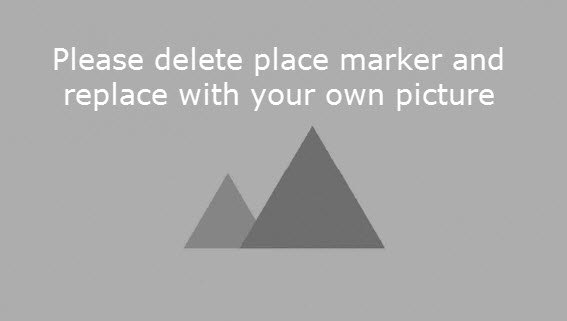
\includegraphics[scale=1.0]{images/placemarker.jpg}			% define cover picture
\end{textblock}

\begin{textblock}{154}(28,135)
	\begin{picture}(150,2)
		\put(0,0){\color{bfhgrey}\rule{150mm}{2mm}}
	\end{picture}
\end{textblock}
\color{black}

% Institution / titel / subtitel / authors / experts:
%---------------------------------------------------------------------------
\begin{flushleft}

\vspace*{115mm}

\fontsize{26pt}{28pt}\selectfont 
\heading				\\							% Read heading from file leader/title.tex
\vspace{2mm}

\fontsize{16pt}{20pt}\selectfont\vspace{0.3em}
Place your subheading here 			\\				% Insert subheading
\vspace{5mm}

\fontsize{10pt}{12pt}\selectfont
\textbf{Description of thesis (semester- / Bachelor thesis / etc.)} \\		% Insert text
\vspace{3mm}

% Abstract (eingeben):
%---------------------------------------------------------------------------
\begin{textblock}{150}(28,190)
\fontsize{10pt}{12pt}\selectfont
[Insert short text (abstract) if desired] \\ 
This document serves as a template for the compilation of reports according to the guidelines of the BFH. The template is written in LATEX and supports the automatic writing of various directories, references, indexing and glossaries. This small text is a summary of this document with a length of 4 to max. 8 lines. \\ 
The cover picture may be turned on or off in the lines 157/158 of the file template.tex.
\end{textblock}

\begin{textblock}{150}(28,225)
\fontsize{10pt}{17pt}\selectfont
\begin{tabbing}
xxxxxxxxxxxxxxx\=xxxxxxxxxxxxxxxxxxxxxxxxxxxxxxxxxxxxxxxxxxxxxxx \kill
Degree course:	\> [z.B. Electrical and Communication Engineering]	\\		% insert name of degree course
Authors:		\> [Test Peter, M\"uster R\"os\"a]		\\					% insert names
Tutor:	\> [Dr.~Xxxx Xxxx, Dr.~Yyyy Yyyy]		\\							% insert names
Constituent:	\> [Wwwww AG]					\\							% insert names
Experts:		\> [Dr.~Zzzz Zzzz]				\\							% insert names
Date:			\> \versiondate					\\							% read from file leader/version.tex
\end{tabbing}

\end{textblock}
\end{flushleft}

\begin{textblock}{150}(28,280)
\noindent 
\color{bfhgrey}\fontsize{9pt}{10pt}\selectfont
Berner Fachhochschule | Haute \'ecole sp\'ecialis\'ee bernoise | Bern University of Applied Sciences
\color{black}\selectfont
\end{textblock}


\end{titlepage}

%
% ===========================================================================
% EOF
%
		% activate for frontpage with picture
% Control of versions :
% -----------------------------------------------

\begin{textblock}{180}(15,150)
\color{black}
\begin{huge}
Versions
\end{huge}
\vspace{10mm}

\fontsize{10pt}{18pt}\selectfont
\begin{tabbing}
xxxxxxxxxxx\=xxxxxxxxxxxxxxx\=xxxxxxxxxxxxxx\=xxxxxxxxxxxxxxxxxxxxxxxxxxxxxxxxxxxxxxxxxxxxxxx \kill
Version	\> Date	\> Status			\> Remarks		\\
0.1	\> 01.08.2013	\> Draft		\> Lorem ipsum dolor sit amet	\\	
0.2	\> 21.08.2013	\> Draft		\> Phasellus scelerisque	\\ 
0.3	\> 02.09.2013	\> Draft		\> Donec eget aliquam urna. Lorem ipsum dolor sit amet	\\ 
1.0	\> 26.01.2014	\> Final		\> Lorem ipsum dolor sit ametPhasellus scelerisque, leo sed iaculis ornare 	\\ 
1.1	\> 31.01.2014	\> Correction	\> Layout changed	\\
1.2	\> 07.02.2014	\> Addition		\> Chapter 1.1 extended	\\
\end{tabbing}

\end{textblock}

\cleardoubleemptypage
\setcounter{page}{1}
\cleardoublepage
\phantomsection 
\addcontentsline{toc}{chapter}{Abstract}
\chapter*{Abstract}
\label{chap:abstract}

In this thesis we try to verify some properties of Bitcoin-S.

First, we look at some theory about formal verification, Stainless -- a verification tool and Bitcoin-S -- an open source implementation of the Bitcoin protocol.

Then, we try to verify that a non-coinbase transaction should not generate new coins.
We create a transaction and check it in Bitcoin-S.
After some time we realize that it is not possible with the current tools and the given time.
But because we familiarized us with the Bitcoin-S code we find a bug and send a bug fix to the Bitcoin-S project.

So we verify a less interesting property property of Bitcoin-S.
There is a datatype Satoshis that represents bitcoins. We verify that the addition of Satoshis with zero results in the same amount of Satoshis.
Even this needs many changes in the code that we go through step-by-step.

Finally, we see that software should be written with verification tools in mind, because otherwise the code possibly must be rewritten when it comes to verification.

\cleardoubleemptypage
%---------------------------------------------------------------------------

% Table of contents
%---------------------------------------------------------------------------
\tableofcontents
\cleardoublepage
%---------------------------------------------------------------------------

% Main part:
%---------------------------------------------------------------------------
\pagenumbering{arabic}

\chapter{Introduction}
\label{chap:introduction}

The longer and more complex a source code is, the more difficult it is to verify its correctness.
There are different approaches to show the correctness of a program.
One of them is formal verification.
In contrast to testing, where only predefined inputs are tested, with formal verification all possible inputs are covered.
The correctness of a program is analyzed relative to its formal specification.
Formal specification is a mathematical description of a software behavior that can be used by the verification tool to verify the code.
We will see an example of a formal specification shortly.

In this work we use the verification framework Stainless to verify parts of the code of Bitcoin-S, a Scala implementation of the Bitcoin protocol.
In the following we look at the main aspects of formal verification with Stainless and properties of Bitcoin-S we want to verify.


\section{Formal verification with Stainless}
\label{sec:stainless}

Stainless is developed by "Lab for Automated Reasoning and Analysis" (LARA) at EPFL's School of Computer and Communication Sciences.
Using this framework we can verify the correctness of Scala programs.
The following overview of the framework is taken from the section \href{https://epfl-lara.github.io/stainless/intro.html}{Introduction} of the Stainless documentation \cite{Stainless:documentation}.

Stainless statically verifies that a program satisfies a given specification and that a program will not crash at runtime.
The framework covers all possible inputs and finds a counter examples for possible failures in a program which violate the given specification.

The main functions used to write a specification are \textit{require} and \textit{ensuring}.

With \textit{require} we define a precondition of a function, which we want to verify.
\textit{require} is placed at the beginning of the function body.
\textit{require} specifies, if the parameter of the function hold a certain condition.

With \textit{ensuring}, we define the postcondition of a function.
\textit{ensuring} is placed at the end of the function after the body.
\textit{ensuting} specifies, if the return value or the result of the function hold a certain condition.

On invoking Stainless, it tries to prove that the postcondition always holds, assuming the given precondition does hold.

The following example demonstrates a simple formal specification for the function calculating factorial.
This is a modified example from the section \href{https://epfl-lara.github.io/stainless/intro.html}{Introduction} of the Stainless documentation \cite{Stainless:documentation}, so Stainless reports an error verifying it.
\begin{lstlisting}[language=Scala]
  def factorial(n: Int): Int = {
      require(n >= 0)
      if (n == 0) {
        1
      } else {
        n * factorial(n - 1)
      }
  } ensuring(res => res >= 0)
\end{lstlisting}

The function recursively calculates factorial of an integer number.
The input of the function is constrained with \textit{require} to a non-negative value.
The result should also be non-negative.
Thus, Stainless will verify whether the result of the factorial calculation is non-negative for all non-negative inputs.

Stainless can produce 3 outcomes of postcondition verification: \textit{valid}, \textit{invalid} and \textit{unknown}.
If the postcondition is \textit{valid} Stainless could prove that for any inputs constrained in the precondition, the postcondition always holds.
Reporting the postcondition as \textit{invalid} the framework could find at least one counterexample which satisfies the precondition but violates the postcondition.
If Stainless is unable to prove the postcondition or find a counterexample it reports the outcome \textit{unknown}.
In this case a timeout or an internal error occurred.
Furthermore, Stainless checks for calls in the code to the function with invalid arguments violating the precondition.
For example if we invoke factorial with a negative number it reports \textit{invalid}.

Let's return back to our incorrect example with factorial.
Stainless reports the following result for the factorial verification from our example:
\begin{figure}[H]
	\centering
		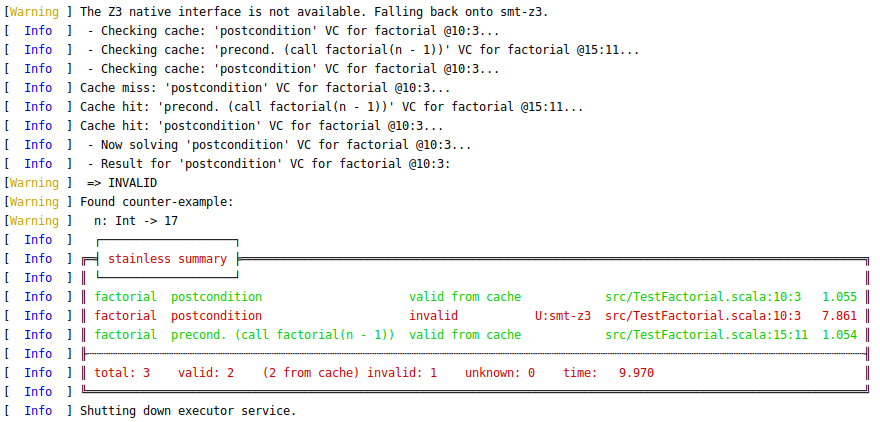
\includegraphics[scale=0.5]{images/output1.png}
	\caption{Output of Stainless verification for calculating factorial of Int number}
	\label{fig:output1}
\end{figure}

Stainless disproves the postcondition and gives the number 17 as a counterexample.
Due to an overflow in the 32 bit Int the result becomes a negative value.
The program would work correct by changing the type from Int to BigInt.

Stainless supports only a subset of Scala.
They call is Pure Scala.
You can find the specification of Pure Scala on the Stainless documentation website \cite{Stainless:documentation} in the section \href{https://epfl-lara.github.io/stainless/purescala.html}{Pure Scala}.

In addition, Stainless has its own library with annotations, reimplementaion of some core data types, collections and input-output functions and more.
Some of them are described on the website in the section \href{https://epfl-lara.github.io/stainless/library.html}{Stainless Library}.
There are more details about library in the source code of Stainless on GitHub \cite{Stainless:github} in the folder \href{https://github.com/epfl-lara/stainless/tree/master/frontends/library/stainless}{\textit{frontends/library/stainless}}.

Stainless verifies Scala programs using SMT (satisfiability modulo theories) solvers. 


\section{The Properties to Verify}

Bitcoin-S is a large project found on GitHub implementing many functionalities.
In this work we look at two of them, namely the \nameref{property_1} and the \nameref{property_2} described shortly.
Thus, we go through the relevant code parts to verify those properties, look at some challenges with Stainless and see why we should write software with verification in mind.
We will rewrite the code to Pure Scala, because Bitcoin-S is not written in it.


\subsection{No Inflation Property}
\label{property_1}



\subsection{Addition with Zero Property}
\label{property_2}



\chapter{Using Stainless}
\label{chap:using_stainless}
This chapter describes the setup and integration process of Stainless in a new or already existing project.
It also shows the compatibility of Stainless with Scala as Stainless supports only a purely functional subset of Scala which they call \emph{Pure Scala}.

\section{Configuration}
There are two ways to integrate Stainless in a Scala project, the scala build tool (abt) plugin or a command line tool.
Both, when run, analyses the passed code and report warnings to the console about the given code.
Stainless requires and Scala recommends Java SE Development Kit 8.
Newer Java versions won't compile.

\subsection{sbt}
sbt for Scala is like gradle or maven for Java.
It can compile Scala code continously or manual, manage dependencies with support for Maven-formatted repositories, mixing Scala and Java projects and much more.

A simple sbt project has the following structure:
\dirtree{%
  .1 ..
  .2 project.
  .3 build.properties.
  .3 plugins.sbt.
  .2 src.
  .3 main.
  .4 scala.
  .5 Main.scala.
  .2 build.sbt.
}
\emph{build.properties} specifies the abt version used for this project.
If the version is not available locally, sbt will download it.

In \emph{plugins.sbt} new sbt plugins can be added.
A plugin extends the build definition.
Mostly this means adding and overriding settings.

\emph{build.sbt} defines the build definition.
There can be several projects or subprojects as sbt doc calls it.

Here an example for a single project in \emph{build.sbt}:
\begin{lstlisting}[language=scala]
scalaVersion := "2.12.8"

lazy val root = (project in file("."))
\end{lstlisting}
The project is called root and its source files are located in the files directory.
Executing \code{sbt compile} should now compile the code.

The Stainless webpage has a guide on how to integrate Stainless in an existing project.
The simplifies steps are:
\begin{itemize}
  \item Install an external solver.
  \item Add Stainless sbt plugin to \emph{plugins.sbt}
  \item Enable the plugin in \emph{build.sbt} for the project.
\end{itemize}
After this setup, Stainless will report errors to the console, when running \code{sbt compile}.

\subsection{Command Line Tool}
There are two ways to use the command line tool.

Either download a prebuilt JAR file from efpl-lara/stainless GitHub repository or built a binary from source.
The prebuild versions are released by Stainless.
The latest was released on January 14, when there was no support for Scala 2.12.
The 'Bump Scala to 2.12.8' branch was merged on March 4.

If latest features are needed, like support for Scala 2.12, the build from source is required.
Here a short installation description.
Full description can be found on the Stainless documentation pages.
\begin{itemize}
  \item Install sbt.
  \item Check out GitHub repository.
  \item Run \code{sbt universal:stage} inside the project.
\end{itemize}
This generates \emph{frontends/scalac/target/universal/stage/bin/stainless-scalac}.

To check the source code with one of those either \code{java -jar downloaded.jar source.scala} or \code{stainless-scalac source.scala} must be invoked.
The file \emph{source.scala} is the file to be checked.

As compiling without a build tool, this command will become really complex for bigger projects.
All dependencies must be on the classpath and all source files appended.
Those are added with \code{-classpath Dep1.jar:Dep2.jar:...:DepN.jar src1.scala src2.scala ... srcM.scala}.

\section{Scala compatibility (Pure Scala, imperative features, dedicated BigInt, Generics...)}
Stainless supports only a subset of Scala.
They call it Pure Scala.
We will see some of this restrictions we have detected during this work in the next chapter.
There is a list of what's supported in the Stainless documentation.

\chapter{Using Bitcoin-S-Core}
\label{chap:using_bitcoins}
This chapter describes the relevant parts needed to verify that a non-coinbase transaction cannot generate new coins in Bitcoin-S-Core.
We will see, how to create valid and invalid transactions with Bitcoin-S-Core and how this transactions are validated against the described property.

\section{Creation of a Transaction}
Some parts of the code in this section are from Bitcoin-S-Core transaction builder example.\cite{BitcoinSCore:txbuilderexample}
Bitcoin-S-Core has a bitcoin transcation builder class with the following signature:
\begin{lstlisting}[language=scala]
  BitcoinTxBuilder(
    destinations: Seq[TransactionOutput], // where we send money
    utxos: BitcoinTxBuilder.UTXOMap,      // unspent transaction outputs
    feeRate: FeeUnit,                     // fee rate per byte
    changeSPK: ScriptPubKey,              // public key
    network: BitcoinNetwork               // bitcoin network information
  ): Future[BitcoinTxBuilder]             // sign TxBuilder to get tx
\end{lstlisting}
Here is how those parameters are generated.

First, a previous transaction with outputs is needed to spend some money from.
This is created here, to show the process.
It could also be parsed from a transaction in the bitcoin network.
A single output is sufficient for this example.
So, first create a new keypair to sign the next transaction and have a scriptPubKey where the money is.
Then define the amount to spend (here 10000 Satishis) collect this information in a transaction output and add it to the previous transaction.
\begin{lstlisting}[language=scala]
  val privKey = ECPrivateKey.freshPrivateKey
  val creditingSPK = P2PKHScriptPubKey(pubKey = privKey.publicKey)

  val amount = Satoshis(Int64(10000))

  val utxo = TransactionOutput(currencyUnit = amount, scriptPubKey = creditingSPK)

  val prevTx = BaseTransaction(
    version = Int32.one,
    inputs = List.empty,
    outputs = List(utxo),
    lockTime = UInt32.zero
  )
\end{lstlisting}
Next, the new transaction should point to an output of the previous transaction.
Thus, a outpoint is created with the id of the previous transaction and the index pointing to the specific output of it.
This is collected in an utxo spending info which is then put in the list of all utxos (only one here).
\begin{lstlisting}  
  val outPoint = TransactionOutPoint(prevTx.txId, UInt32.zero)

  val utxoSpendingInfo = BitcoinUTXOSpendingInfo(
    outPoint = outPoint,
    output = utxo,
    signers = List(privKey),
    redeemScriptOpt = None,
    scriptWitnessOpt = None,
    hashType = HashType.sigHashAll
  )

  val utxos = List(utxoSpendingInfo)
\end{lstlisting}
Then, the destination, where the money goes, is defined.
This includes a destination script pub key, as well as a the amount to spend to it.
\begin{lstlisting}
  val destinationAmount = Satoshis(Int64(5000))

  val destinationSPK = P2PKHScriptPubKey(pubKey = ECPrivateKey.freshPrivateKey.publicKey)

  val destinations = List(
    TransactionOutput(currencyUnit = destinationAmount, scriptPubKey = destinationSPK)
  )
\end{lstlisting}
Finally. define a fee rate, the network params and create a transaction builder.
\begin{lstlisting}
  val feeRate = SatoshisPerByte(Satoshis.one)

  val networkParams = RegTest // soem static values for testing

  val txBuilder: Future[BitcoinTxBuilder] = BitcoinTxBuilder(
    destinations = destinations,
    utxos = utxos,
    feeRate = feeRate,
    changeSPK = creditingSPK,
    network = networkParams
  )
\end{lstlisting}
After calling sign on the transaction builder a valid transaction is returned.
\begin{lstlisting}
  val signedTxF: Future[Transaction] = txBuilder
    .flatMap(_.sign)
    .map {
      (tx: Transaction) => println(tx.hex) // transaction in hex for the bitcoin network
    }
\end{lstlisting}
There is no need for a transaction input, since a transaction out point is kind of the pointer to a transaction input.

\section{Validation of a Transaction}
Bitcoin-S-Core offers a function called \emph{checkTransaction}.
This is its type signature.
\begin{lstlisting}
  checkTransaction(transaction: Transaction): Boolean
\end{lstlisting}
It takes a transaction as input and returns a boolean whether the transaction is valid or not.
So for example when passing the built tx from above to this function the returned value would be true.
There are several checks in checkTransaction.
For example it checks if there is either no input or no output.
In this case it returns false.

The relevant parts for the property to be verified are the following two lines.
\begin{lstlisting}
  val prevOutputTxIds = transaction.inputs.map(_.previousOutput.txId)
  val noDuplicateInputs = prevOutputTxIds.distinct.size == prevOutputTxIds.size
\end{lstlisting}
It gathers all inputs output transaction ids.
On this previous outputs ids it calls distinct and checks if the size stays the same.
Distinct removes duplicates, so if there was two times the same input transaction id the size of those ids would be greater before calling distinct.

There is a bug in those two lines, as described in the next chapter.

\chapter{Towards verifyng Bitcoin-S with Stainless}
\label{chap:connecting}

\section{Integration (Versionskonflikte, neues Plugin)}


\section{Error Reporting with sbt and JAR}


\section{Trying to Verify checkTransaction}

\subsection{Findings}


\subsection{Bugfix}


\section{Verification of Method "+ 0" // Change this}
After so many failures, we have decided to search for the smallest unit in Bitcoin-S-Core that is worthwhile to verify.
We found the addition of two Satoshis would be a good candidate.
To make it even more easy, we decided to verify only the addition, where we add zero to an amount of Satoshis.
The signature looks like the following.
\begin{lstlisting}
  +(c: CurrencyUnit): CurrencyUnit
\end{lstlisting}
Where the class Satoshis extends CurrencyUnit.
The post condition would be, that the parameter c must be zero.
\begin{lstlisting}
  require(c.satoshis.underlying == Int64.zero)
\end{lstlisting}
\emph{c.satoshis} is an abstract method of CurrencyUnit that must return an instance of the class Satoshis.

\emph{c.satoshis.underlying} is also an abstract method of CurrencyUnit that must return an instance of the abstract type A.

Both are implemented in Satoshis where A is set to Int64.
So the underlying number of the parameter must be zero.

Next we ensure, that the result is the same value as \emph{this}.
\begin{lstlisting}
  ensuring(res => res.satoshis == this.satoshis)
\end{lstlisting}
Here, we can directly use equals (==) on Satoshis, because its a case class and Int64, the only parameter of Satoshis is a case class too.

After writing the verification, we ran Stainless on the source files.
It prints a lot of errors because of code incompatibility.
So we had to rewrite it as described in the following sections.

\subsection{Rewriting Abstract Type Member}
Stainless output:
\begin{lstlisting}
[ Error  ] CurrencyUnits.scala:5:3: Stainless doesn't support abstract type members
           type A
\end{lstlisting}
This should be easy to rewrite by using generics instead of an abstract type, right?
Unfortunately not.
The problem is, CurrencyUnit uses its implementing class Satoshis.

Simplified code.
\begin{lstlisting}
  sealed abstract class CurrencyUnit {
    def +(c: CurrencyUnit): CurrencyUnit =
      Satoshis(satoshis.underlying + c.satoshis.underlying)
  }

  sealed abstract class Satoshis extends CurrencyUnit
\end{lstlisting}
Thus, changeing it to generics, Satoshis is not of type CurrencyUnit anymore and neither of type CurrencyUnit[A], where A is the new generic type.
Satoshis extends CurrencyUnit with type Int64, so it is of type CurrencyUnit[Int64].
That's to specific.

Since there is no easy way to fix it and the code should stay as much as possible the original, removing the abstract type might be the only choice.
The verification is a bit more limited, to only Satoshis, but that's no problem, because the goal is to verify the addition of Satoshis.

So by removing the abstract type and fix it to Int64 as defined by Satoshis, there was one error less in Stainless.

\subsection{Rewriting Generics}
// I dont understand this.. maybe just a missing feature in Stainless?
Stainless output:
\begin{lstlisting}
  [ Error  ] NumberType.scala:3:30: Unknown type parameter type T
             sealed abstract class Number[T <: Number[T]]

\end{lstlisting}

\begin{lstlisting}
  sealed abstract class Number[T <: Number[T]] extends BasicArithmetic[T]  
\end{lstlisting}

\subsection{Rewriting Objects}
// TODO reason?

Stainless output:
\begin{lstlisting}
[ Error  ] CurrencyUnits.scala:54:1: Objects cannot extend classes or implement
           traits, use a case object instead
           object Satoshis extends BaseNumbers[Satoshis] {
\end{lstlisting}
Changing the objects that extends classes to case objects solves this problem.

\subsection{Rewriting BigInt Constructor (only literal argument, no long argument, etc.)}
Stainless output:
\begin{lstlisting}
[ Error  ] CurrencyUnits.scala:47:33: Only literal arguments are allowed for BigInt.
           def toBigInt: BigInt = BigInt(toLong)
\end{lstlisting}
As described before, Stainless supports only a subset of Scala.
They provide their own dedicated BigInt library.
This library does not have support for dynamic BigInt construction only for string literals.

Again, a simplified version.
\begin{lstlisting}
  sealed abstract class Satoshis extends CurrencyUnit {
    def toBigInt: BigInt = BigInt(toLong)
    def toLong: Long = underlying.toLong
  }

  object Int64 extends BaseNumbers[Int64] {
    private case class Int64Impl(underlying: BigInt) extends Int64
  }
\end{lstlisting}
This would be really hard to refactor, because Bitcoin-S-Core tries to be as much dynamic as possible so it can be used with other cryptocurrencies too.
Maybe it would even be impossible, because they need to parse a lot from the bitcoin network.

Restricting the code one more time helps.
\emph{toBigInt} can directly return underlying, because in case of Int64, which is what Satoshis use, it is a BigInt.
So it does not be converted from BigInt to Long and back to BigInt.

\subsection{Rewriting Private Inner Classes}
Stainless output (simplified):
\begin{lstlisting}
  [Warning ] CurrencyUnits.scala:36:3: Could not extract tree in class:
             case private class SatoshisImpl extends Satoshis
\end{lstlisting}
Stainless is not able to extract private classes inside other objects.
Bitcoin-S-core uses it a lot, because they separate the class from its implementation.
\begin{lstlisting}
  object Int64 extends BaseNumbers[Int64] {
    private case class Int64Impl(underlying: BigInt) extends Int64 
  }
\end{lstlisting}
This is an easy one.
Just extract the inner class out of the object.
This is not exactly the same code but since the class is still private it can not be extended outside of the file.

\subsection{Rewriting Type Member}
Stainless output:
\begin{lstlisting}
  [Warning ] NumberType.scala:5:3: Could not extract tree in class: type A
             = BigInt (class scala.reflect.internal.Trees$TypeDef)
             type A = BigInt
\end{lstlisting}
Since the type A is not overridden in any of its subclasses, this can simply be hard coded.
\begin{lstlisting}
  sealed abstract class Number {
    type A = BigInt
    protected def underlying: A
    def apply: A => T
  }
\end{lstlisting}
Replace every occurence of A with BigInt.
This might be a missing feature in Stainless that should not be to hard to fix.
There is an open pull request \mypound470 on Github for this issue.

\subsection{Rewriting Usage of BigInt \&-Function}
Stainless output:
\begin{lstlisting}
  [ Error  ] NumberType.scala:19:14: Unknown call to & on result (BigInt) with
             arguments List(Number.this.andMask) of type List(BigInt)
             require((result & andMask) == result,
\end{lstlisting}
Due to the restrictions on BigInt, the \& function on it is not supported too.
\begin{lstlisting}
  sealed abstract class Number extends BasicArithmetic[Int64] {
    def andMask: BigInt

    override def +(num: Int64): Int64 = apply(checkResult(underlying + num.underlying))

    private def checkResult(result: BigInt): BigInt = {
      require((result & andMask) == result, "Result was out of bounds, got: " + result)
      result
    }
  }
\end{lstlisting}
This is a bound check.
It checks, if the result of the addition is in range of the specified type (Int64 here).
So here the \& mask can be replaced with a bound check whether the result is in range of Long.MinValue and Long.MaxValue.
Again the code gets a bit more static but for this usecase its ok.

\subsection{Rewriting require}
Stainless output:
\begin{lstlisting}
  [Warning ] NumberType.scala:54:3: Could not extract tree in class:
             scala.this.Predef.require(Int64Impl.this.underlying.<=(
             math.this.BigInt.long2bigInt(9223372036854775807L)),
             "Number was too big for a int64, got: ".+(Int64Impl.this.underlying))
             (class scala.reflect.internal.Trees$Apply)
             require(underlying <= 9223372036854775807L,
\end{lstlisting}
This is, because Stainless does not support require with a second String parameter.
Removing this String fixes the error.

\subsection{Propagate require}
Finally the code works with Stainless.
But there is another problem.
Bitcoin-S-Core uses require like a fail-fast method where as Stainless needs it to verify the code.

Stainless output:
\begin{lstlisting}
  [Warning ] Found counter-example:
  [Warning ]   thiss: { x: Object | @unchecked isNumber(x) } -> Int64Impl(0)
  [Warning ]   num: { x: Object | @unchecked isInt64(x) }    -> 
                 Int64Impl(9223372036854775808)
\end{lstlisting}
Corresponding code:
\begin{lstlisting}
  sealed abstract class Number extends BasicArithmetic[Int64] {
    override def +(num: Int64): Int64 = apply(checkResult(underlying + num.underlying))

    private def checkResult(result: BigInt): BigInt = {
      require(
        result <= BigInt("9223372036854775807")
        && result >= BigInt("-9223372036854775808")
      )
      result
    }
  }
\end{lstlisting}
But how can Stainless find a counter example ignoring the require in checkResult?
Since Stainless is a static verification tool, it tests every possibility.
So it can use a number bigger than the maximum Int64 and pass it to the addition.
The require in checkResult will then fail.
Thus, the addition need to have the restrictions of checkResult too.
\begin{lstlisting}
  override def +(num: Int64): Int64 = {
    require(
      num.underlying <= BigInt("9223372036854775807")
      && num.underlying >= BigInt("-9223372036854775808")
      && this.underlying <= BigInt("9223372036854775807")
      && this.underlying >= BigInt("-9223372036854775808")
    )
    apply(checkResult(underlying + num.underlying))
  }
\end{lstlisting}
Stainless finds another counter example:
\begin{lstlisting}
  [Warning ] Found counter-example:
  [Warning ]   num: { x: Object | @unchecked isInt64(x) }    -> Int64Impl(1)
  [Warning ]   thiss: { x: Object | @unchecked isNumber(x) } ->
                 Int64Impl(9223372036854775807)
\end{lstlisting}
Sure, it can just add one to the maximum Int64 and the require does not hold anymore.
The goal is to check the addition of zero so lets add a restriction for num to be zero.

Finally, it works and verifies correctly.

\section{Result}
\begin{figure}[H]
	\centering
		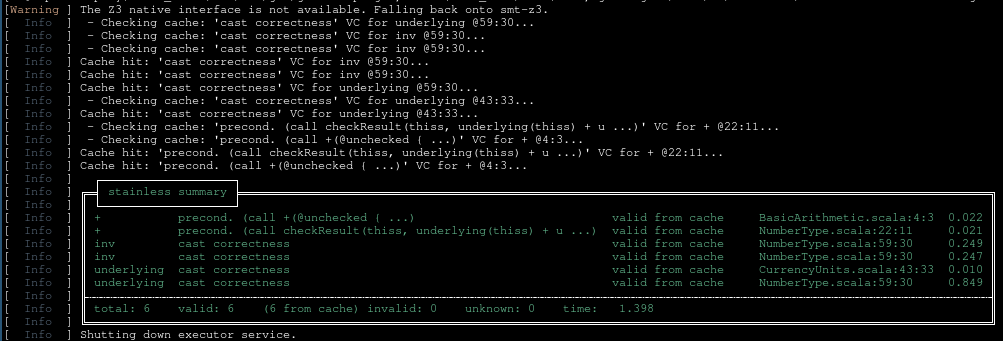
\includegraphics[scale=0.45]{images/final_verify_output.png}
	\caption{Output of Stainless verification for addition with 0 of Bitcoin-S-Cores CurrencyUnit}
	\label{fig:output1}
\end{figure}

\chapter{Conclusion}
\label{chap:conclusion}

Because of the limitations of the verication tool, we could only verify a rewritten version of the original Bitcoin-S code.
So we can not guarantee the correctness of the addition of Satoshis with zero in Bitcoin-S.
Not all changes we made were as trivial as the replacement of objects with case objects.
For these non-trivial changes, as seen for example the bound check in section \ref{sec:bound_check}, we cannot say whether they are equivalent to the original implementation or not.

So code should be written specically with formal verication in mind, in order to successfully verify it.
Otherwise, it needs a lot of changes in the software because verification is mathematical and the current software is written mostly in object-oriented style.
Software written in the functional paradigm would be much easier to reason about.

Thus, either Stainless must find ways to translate more of built-in object-oriented patterns of Scala to their verification tool or developers must invest more in functional programming.

Also, we found that trying to verify code reveals bugs as shown in section \ref{sec:bugfix}.
Finally, our work led to some feedback to the Stainless developers to improve the tool.

%---------------------------------------------------------------------------

% Selbständigkeitserklärung
%---------------------------------------------------------------------------
\cleardoublepage
\phantomsection 
\addcontentsline{toc}{chapter}{Declaration of authorship}
\chapter*{Declaration of primary authorship}
\label{chap:declaration_authorship}

\vspace*{10mm} 

We hereby confirm that we have written this thesis independently and without using other sources and resources than those specified in the bibliography.
All text passages which were not written by me are marked as quotations and provided with the exact indication of its origin. 

\vspace{15mm}

\begin{tabbing}
xxxxxxxxxxxxxxxxxxxxxxxxxxxxxx\=xxxxxxxxxxxxxxxxxxxxxxxxxxxxxx\=xxxxxxxxxxxxxxxxxxxxxxxxxxxxxx\kill
Place, Date:		\> Biel, \versiondate \\ \\ 
Last Names, First Names:	\> Doukmak Anna 	\> Boss Ramon \\ \\ \\ \\ 
Signatures:	\> ......................................\> ...................................... \\
\end{tabbing}

%---------------------------------------------------------------------------

% Glossary
%---------------------------------------------------------------------------
\cleardoublepage
\phantomsection 
\addcontentsline{toc}{chapter}{Glossay}
%\renewcommand{\glossaryname}{Glossay}
\printglossary
%---------------------------------------------------------------------------

% Bibliography
%---------------------------------------------------------------------------
\cleardoublepage
\phantomsection 
\addcontentsline{toc}{chapter}{Bibliography}
\bibliographystyle{IEEEtranS}
\bibliography{database/bibliography}{}
%---------------------------------------------------------------------------

% Listings
%---------------------------------------------------------------------------
\cleardoublepage
\phantomsection 
\addcontentsline{toc}{chapter}{List of figures}
\listoffigures
\cleardoublepage
\phantomsection 
\addcontentsline{toc}{chapter}{List fo tables}
\listoftables
%---------------------------------------------------------------------------

% Index
%---------------------------------------------------------------------------
\cleardoublepage
\phantomsection 
\addcontentsline{toc}{chapter}{Index}
\printindex
%---------------------------------------------------------------------------

% Attachment:
%---------------------------------------------------------------------------
\appendix
\settocdepth{section}
\chapter{Arbitrary Appendix}
\label{chap:appendix_arb}
\endgroup

The European languages are members of the same family. Their separate existence is a myth. For science, music, sport, etc, Europe uses the same vocabulary. The languages only differ in their grammar, their pronunciation and their most common words. Everyone realizes why a new common language would be desirable: one could refuse to pay expensive translators. To achieve this, it would be necessary to have uniform grammar, pronunciation and more common words. If several languages coalesce, the grammar of the resulting language is more simple and regular than that of the individual languages. The new common language will be more simple and regular than the existing European languages. It will be as simple as Occidental; in fact, it will be Occidental. 
\chapter{Additional Appendix}
\label{chap:appendix_B}

\section{Test 1}
To an English person, it will seem like simplified English, as a skeptical Cambridge friend of mine told me what Occidental is. The European languages are members of the same family. Their separate existence is a myth. For science, music, sport, etc, Europe uses the same vocabulary. The languages only differ in their grammar, their pronunciation and their most common words. Everyone realizes why a new common language would be desirable: one could refuse to pay expensive translators. To achieve this, it would be necessary to have uniform grammar, pronunciation and more common words. If several languages coalesce, the grammar of the resulting language is more simple and regular than that of the individual languages. The new common language will be more simple and regular than the existing European languages. 

\subsection{Environment}
It will be as simple as Occidental; in fact, it will be Occidental. To an English person, it will seem like simplified English, as a skeptical Cambridge friend of mine told me what Occidental is. The European languages are members of the same family. Their separate existence is a myth. For science, music, sport, etc, Europe uses the same vocabulary. The languages only differ in their grammar, their pronunciation and their most common words. Everyone realizes why a new common language would be desirable: one could refuse to pay expensive translators. To achieve this, it would be necessary to have uniform grammar, pronunciation and more common words.
\chapter{Content of CD-ROM}
\label{chap:appendix_CDROM}

Content of the enclosed CD-ROM, directory tree, etc.
%---------------------------------------------------------------------------

%---------------------------------------------------------------------------
\end{document}

